\newcommand\T{\rule{0pt}{2.6ex}}
\newcommand\B{\rule[-1.2ex]{0pt}{0pt}}
\newcommand\TT{\rule{0pt}{4.2ex}}
\newcommand\BB{\rule[-2.4ex]{0pt}{0pt}}
\newcommand\TTT{\rule{0pt}{3.8ex}}


The workhorse template of the LSC-Virgo search pipeline is based on the
stationary-phase approximation to the Fourier transform of the
non-spinning post-Newtonian inspiral~\cite{Droz:1999qx,Allen:2005fk}.
This waveform (referred to as SPA or TaylorF2) has been used in the
search for binary neutron
stars~\cite{Abbott:2003pj,Abbott:2005pe,Abbott:2007xi,Abbott:2009tt}, 
sub-solar mass black holes~\cite{Abbott:2005pf,Abbott:2007xi,Abbott:2009tt}
and stellar mass black holes~\cite{Abbott:2009tt}. The TaylorF2 waveform
is parametrised by the binary's component masses $m_1$ and $m_2$ (or
equivalently the total mass $M = m_1 + m_2$ and the symmetric mass ratio
$\eta = m_1 m_2 / M^2$) and an upper frequency cutoff $f_\mathrm{c}$.
Amplitude evolution is modelled to leading order and phase evolution is
modelled to a specified post-Newtonian order. In this section we investigate
the performance of TaylorF2-based searches on the three simulated LIGO
detectors. Results which include the simulated Virgo detector are described in
the next section.  Several analyses were performed 
which test the ability of TaylorF2 waveforms to detect numerical relativity
signals. The analyses differed in the way the TaylorF2 waveforms or the
template bank were constructed.  The results of these searches are summarised
in Table~\ref{tab:inspiral_results}, each column giving the results from a
different search with a summary of the chosen parameters.  We first describe
the parameters varied between these analyses and then present a more detailed
discussion of the results.

All TaylorF2 NINJA analyses used restricted templates (i.e.~the amplitude is
calculated to leading order), however the phase was calculated to various
different post-Newtonian orders~\cite{Blanchet:2002av}. Phases were computed to
either two~\cite{Blanchet:1996pi,Blanchet:1995ez} or three point five
post-Newtonian order~\cite{Blanchet:2001ax,PhysRevD.71.129902,Blanchet:2004ek}
since these are, respectively, the order currently used in LSC-Virgo
searches~\cite{Abbott:2009tt} and the highest order at which post-Newtonian
corrections are known. After choosing a post-Newtonian order, one chooses a
region of mass-parameter space to cover with the template bank.
Figure~\ref{f:ninjaBanks} shows the boundaries of the template banks used in
the analyses. One search used the range used by the LSC-Virgo ``low-mass''
search \cite{Abbott:2009tt} ($m_1,m_2 \ge  1 M_\odot, M \le 35 M_{\odot}$) and
all other searches used templates with total masses in the range $20 M_\odot
\le M \le 90 M_\odot$.  These boundaries were chosen since there were no
signals in the NINJA data with mass smaller than $36 M_\odot$ and there is
little, if any, inspiral power in the sensitive band of the NINJA data for
signals with $M \gtrsim 100 M_\odot$.  The standard LSC-Virgo template bank
generation code~\cite{Babak:2006ty} restricts template generation to signals
with $\eta \le 0.25$, since it is not possible to invert $M$ and $\eta$ to
obtain real-valued component masses for $\eta > 0.25$. All but one of the
searches enforced this constraint, with the $0.03 \le \eta \le 0.25$ for the
low-mass CBC search and $0.1 \le \eta \le 0.25$ for the other
``physical-$\eta$'' searches. It is, however, possible to generate TaylorF2
waveforms with ``unphysical'' values of $\eta > 0.25$.  In two separate studies
using Goddard and Pretorius waveforms~\cite{Pan:2007nw}, and Caltech-Cornell
waveforms~\cite{Boyle:2009dg} it was observed that match between numerical
signals and TaylorF2 templates could be increased by relaxing the condition
$\eta \le 0.25$. One NINJA contribution uses a template bank with $0.1 \le \eta
\le 1.0$ to explore this.

Finally, it is necessary to specify a cutoff frequency at which to terminate the
TaylorF2 waveform. In the LSC-Virgo analyses, this is chosen to be the
innermost stable circular orbit (ISCO) frequency for a test mass in a
Schwarzschild spacetime 
%
\begin{equation}
\label{f_ISCO}
f_\mathrm{ISCO} = \frac{c^3}{6\sqrt{6}\pi GM}.
\end{equation}
%
This cutoff was chosen as the point beyond which the TaylorF2 waveforms
diverge significantly from the true evolution of the
binary~\cite{Blanchet:2002av}.  More recently, comparisons with numerical
relativity waveforms have shown that extending the waveforms up to higher
frequencies improves the sensitivity of TaylorF2 templates to higher mass
signals~\cite{Pan:2007nw,Boyle:2009dg}. The NINJA TaylorF2 analyses use
templates terminated at the ISCO frequency and two additional cut-off
frequencies: the effective ringdown (ERD) frequency and a weighted
ringdown ending (WRD) frequency. The ERD frequency was obtained by comparing
post-Newtonian models to the Pretorius and Goddard
waveforms~\cite{Pan:2007nw}. The ERD almost coincides with the fundamental
quasi-normal mode frequency of the black hole formed by the merger of an
equal-mass non-spinning black-hole binary. The weighted ringdown ending (WRD)
frequency lies between ISCO and ERD, and was obtained by comparing
TaylorF2 waveforms to the Caltech-Cornell numerical
signals~\cite{Boyle:2009dg}.

\begin{table}
\begin{tabular}{| l || c | c | c | c | c | c | c |}
\hline
\bf{Analysis} \T \B & $(1)$ & $(2)$ & $(3)$ & $(4)$ & $(5)$ & $(6)$ \\ \hline
\bf{Freq. Cutoff} \T \B & ISCO & ISCO & ERD & ERD &  WRD & WRD  \\ 
\hline
\bf{PN Order} & 2 PN & 2 PN & 2 PN & 3.5 PN &  3.5 PN& 3.5 PN  \\
\hline
%\parbox{2.8cm}{
%\bf{Component\\ Mass $M_{\odot}$}} & 1--34 & 10--60 & 10--60 & 10--60 & 10--60 & 10--60 \\ 
%\hline
\bf{Total Mass $M_{\odot}$} \T \B & 2--35 & 20--90 & 20--90 & 20--90 & 20--90 & 20--90  \\ 
\hline
\bf{$\eta$ range} \T \B & 0.03--0.25 & 0.10--0.25 & 0.10--0.25 & 0.10--0.25 & 0.10--0.25 & 0.10--1  \\ 
\hline
\parbox{2.3cm}{
\bf{Found Single\\ (H1, H2, L1)}}\TT \BB  & 69, 66, 75 & 72, 43, 66 & 83, 51, 81 & 91, 56, 87 & 90, 55, 88 & 90, 56, 88 \\ 
\hline
\parbox{2.3cm}{
\bf{Found \\Coincidence }} \TT \BB & 49 & 59 & 79 & 82 &  82 & 84 \\ 
\hline
\parbox{2.5cm}{
\bf{Found Second\\Coincidence}} \TT \BB & 48 & 59 & 77 & 81 &  81 & 81 \\ 
\hline 
\end{tabular}
\caption{{\bf Results of inspiral searches using TaylorF2 templates.}  There were 126
injections performed into the data.  The table above shows the number of
injections which were recovered from the three simulated LIGO detectors (H1, H2 and L1) using various different waveform families,
termination frequencies $f_\mathrm{ISCO}$, $f_\mathrm{ERD}$ and $f_\mathrm{WRD}$ 
(as described in the text), and post-Newtonian orders.} 
\label {tab:inspiral_results}
\end{table}


\begin{figure}
  \begin{center}
  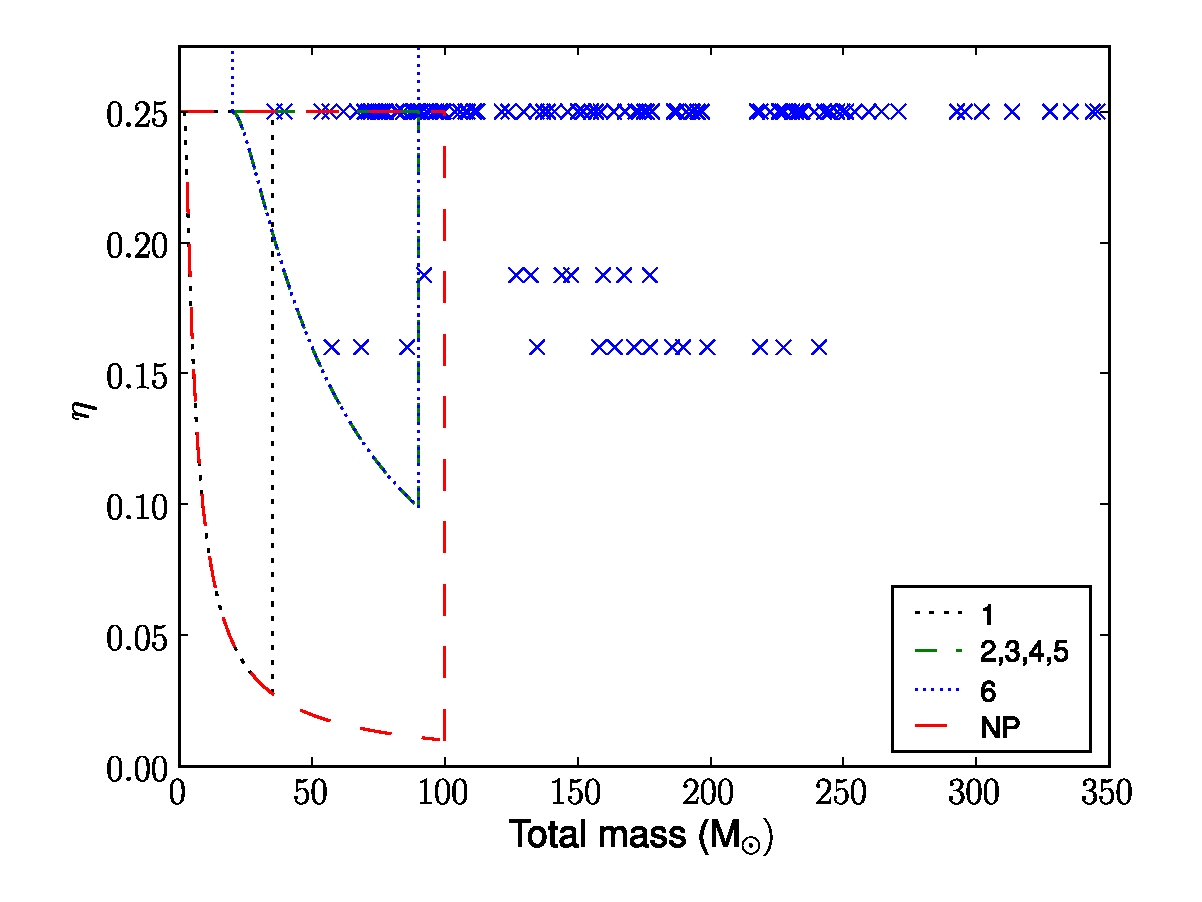
\includegraphics[width=0.8\textwidth]{figures/ninja1/ninja_banks}
  \end{center}
  \caption{{\bf Boundaries of the template banks used in inspiral searches} as a
  function of total mass $M$ and symmetric mass ratio $\eta$. The crosses show
  the location of the injections in the NINJA data set. The numbers in the
  legend correspond to entries in table~\ref{tab:inspiral_results}. Bank 6
  extends in a rectangle up to $\eta = 1.00$, as indicated by the arrows. NP
  is the bank used in the Neyman-Pearson analysis described in 
  Section~\ref{sssec:neyman}.}
  \label{f:ninjaBanks}
\end{figure}

The results of these searches are reported in
Table~\ref{tab:inspiral_results}.  The principal result is the number of
injected signals detected by the search.  For simplicity, we define a
detected signal as one for which there is a candidate gravitational-wave
signal observed within $50$~ms of the coalescence time of the injection,
determined by the maximum gravitational-wave strain of the injected
signal.  We do not impose any additional threshold on the measured SNR or
effective SNR of the candidate.  For a single detector, this will lead
to a small number of falsely identified injections, but for coincidence
results the false alarm rate is so low that we can be confident that the
triggers are associated with the injection. We now describe these
results in the order that they appear in
Table~\ref{tab:inspiral_results}.

Search~$(1)$ used second order post-Newtonian templates terminated at
$f_\mathrm{ISCO}$ with a maximum mass of $M \le 35 M_{\odot}$.  Despite the
fact that no NINJA injections had a mass within the range of this search, a
significant number of signals were still recovered in coincidence both before
and after signal consistency tests.  Although the templates are not a
particularly good match to the injected signals, they are still similar enough
to produce triggers at the time of the injections.  Search~$(2)$ changed the
boundary of the template bank to $20 M_\odot \le M \le 90 M_{\odot}$, but left
all other parameters unchanged.  The number of detected signals increases
significantly as more signals now lie within the mass range searched. 

Search~$(3)$ extended the upper cutoff frequency of the waveforms to
$f_\mathrm{ERD}$. The number of signals detected increased from 59 to 77, as
expected since these waveforms can detect some of the power contained in the
late inspiral or early merger part of the
signal~\cite{Pan:2007nw,Boyle:2009dg}. Search~$(4)$ extends the post-Newtonian
order to 3.5~PN, slightly increasing the number of detected signals to 81.
With the limited number of simulations performed in this first NINJA analysis,
it is difficult to draw a strong conclusion, although there does seem to be
evidence that the higher post-Newtonian order waveforms perform better,
consistent with previous comparisons of post-Newtonian and numerical
relativity waveforms
\cite{Pan:2007nw,Baker:2006ha,Hannam:2007ik,Boyle:2008ge,Boyle:2009dg}.
Search~$(5)$ uses an upper-frequency cutoff of $f_\mathrm{WRD}$ for the
templates. The number of injections found in coincidence for this search is
the same as the search using $3.5$ order templates with a cutoff of
$f_\mathrm{ERD}$, although there are slight differences in the number of found
injections at the single detector level.

Search~$(6)$ extends the template bank of search~$(5)$ to unphysical values of
the symmetric mass ratio. Extending the bank to $\eta\le 1$ increases the
number of templates in the bank by a factor of $\sim 2$. The original and
modified template banks are shown in Figure~\ref{f:templateBanks}. With the
extended template bank the number of injections found in coincidence remains
the same as search~$(5)$ after signal-based vetoes are applied.  However, many
of the injections are recovered at a higher SNR, particular the low-mass
signals, as shown in Figure~\ref{f:templateBanks}.  Some injections show a
reduction in SNR; more work is needed to understand this effect.

\begin{figure}
  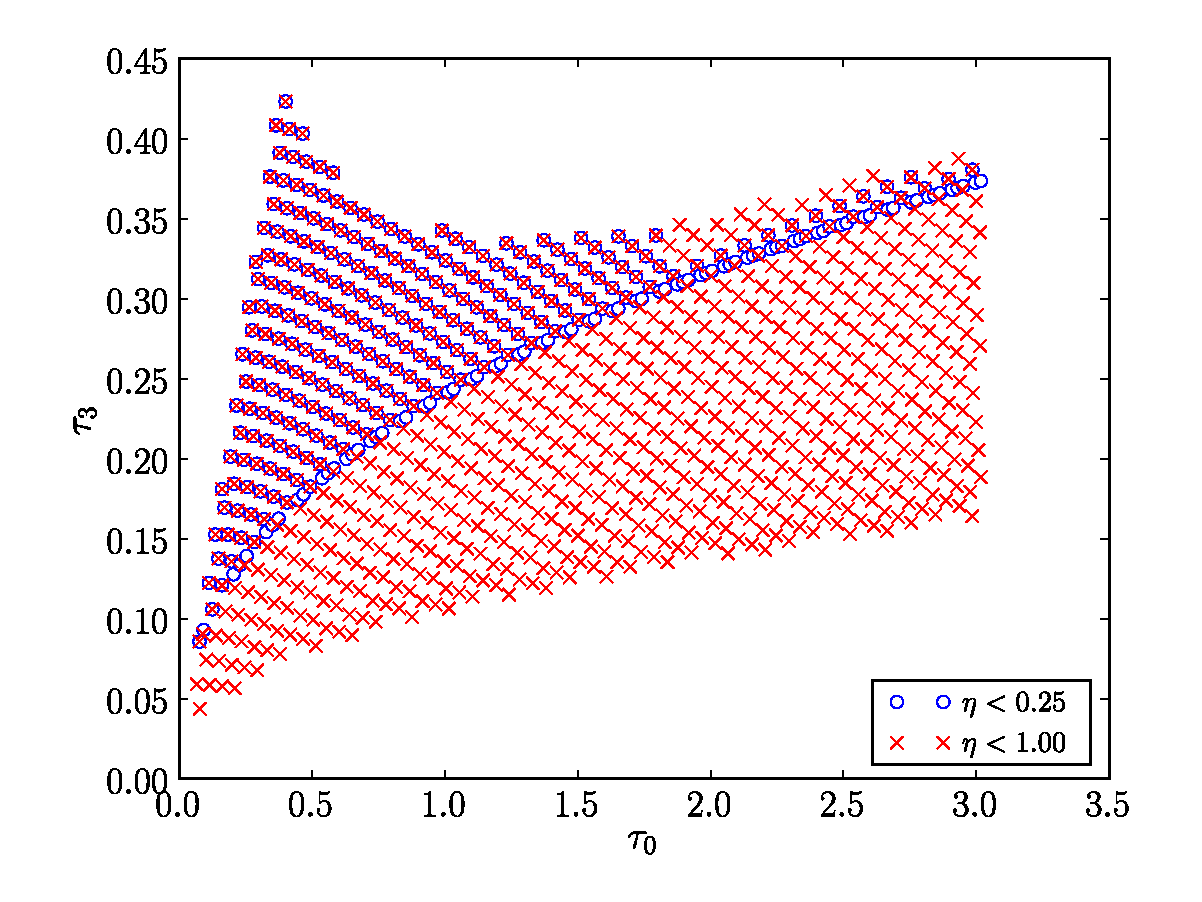
\includegraphics[width=0.50\textwidth]{figures/ninja1/BankBoth}
  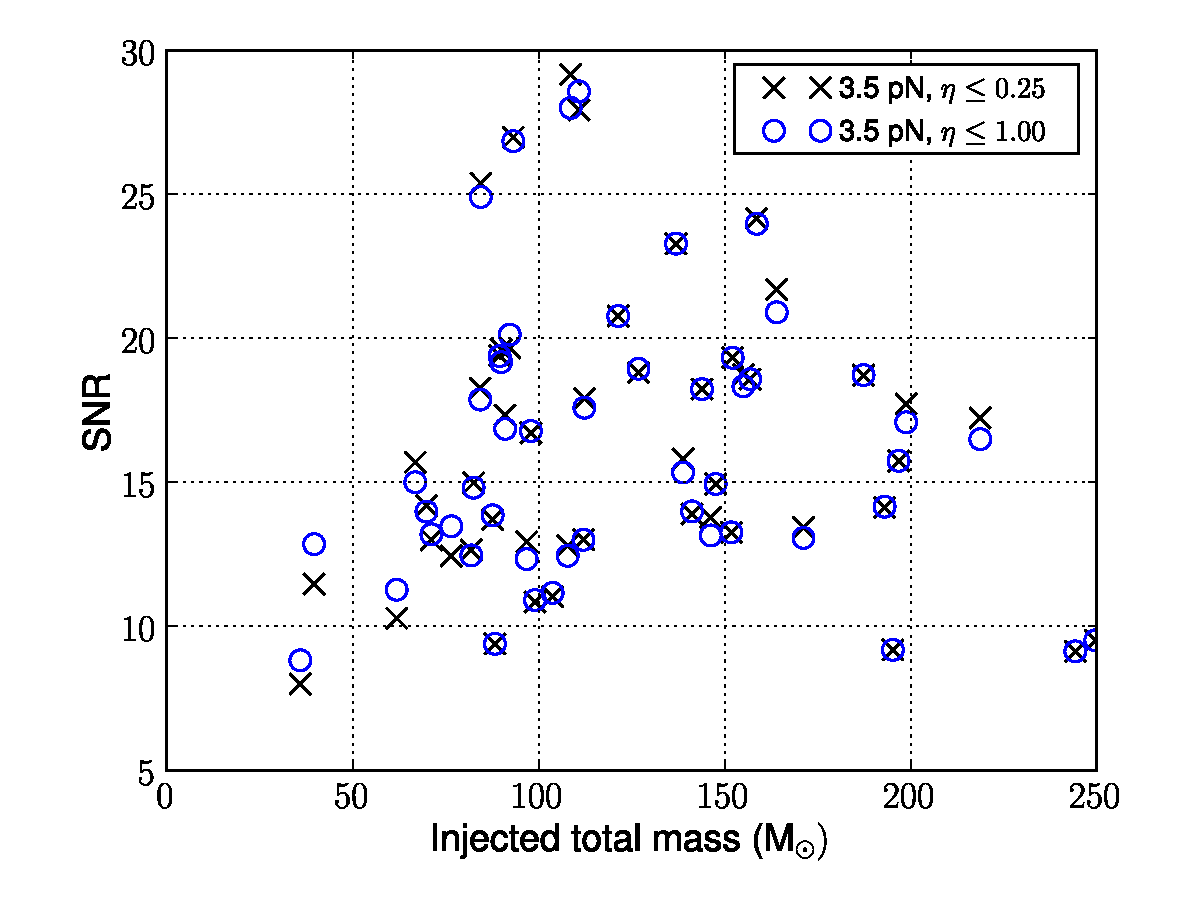
\includegraphics[width=0.50\textwidth]{figures/ninja1/HanfordSNR}
  \caption{{\bf Results from the extended template bank.} 
  {\bf Left:} The template bank generated by the LSC-Virgo
  search pipeline (circles) and the bank obtained by extending to
  $\eta \leq 1.00$ (crosses). In this figure the bank is parametrised
  by $\tau_0$ and $\tau_3$ which are related to the binary masses by
  $\tau_0 = 5M/(256\eta v_0^8)$ and $\tau_3 = \pi M/(8\eta v_0^5)$,
  where $v_0 = (\pi M f_0)^{1/3}$ is a fiducial velocity parameter
  corresponding to a fiducial frequency $f_0 = 40.0 Hz$.
  {\bf Right:} The
  signal-to-noise (SNR) ratio at which NINJA injections were recovered using
  the $\eta \le 0.25$ bank (squares) and the $\eta \le 1$ extended bank
  (circles) in the Hanford detectors, given by $\rho =
  (\rho_\mathrm{H1}^2 + \rho_\mathrm{H2}^2)^{1/2}$. The SNR of the signal
  recovered using the extended bank shows with significant ($> 10\%$) 
  increases over the standard bank for certain injections.}
  \label{f:templateBanks}
\end{figure}

Finally, we note that the majority of signals passed the $\chi^2$
signal-based veto with the thresholds used in the LSC-Virgo pipeline.  The
last two lines of Table~\ref{tab:inspiral_results} show the number of
recovered signals before and after these signal-based vetoes are
performed. The post-Newtonian templates and numerical relativity signals are
similar enough that virtually all of the injected signals survive the signal
based vetoes. 

To illustrate the results of these analyses in more detail, 
Figure~\ref{fig:3_5pn_found_missed} shows which signals were detected and which were
missed by the 3.5 order post-Newtonian TaylorF2 templates terminated at
$f_\mathrm{ERD}$, as a function of injected
total mass and effective distance of the binary (a measure of the
amplitude of the signal in the detector), defined by~\cite{Allen:2005fk}
\begin{equation}
D_\mathrm{eff} = d \left/ \sqrt{F_+^2 (1 + \cos^2 \iota)^2/4 + F_\times^2 \cos^2 \iota}\right.,
\label{eq:effdist}
\end{equation}
where $d$ is the luminosity distance of the binary.

One signal, with total mass of $110 M_{\odot}$ and effective distance $\sim
200$ Mpc, was missed while others with similar parameters were found.  This
signal was one of the Princeton waveforms (labelled \verb|PU-e0.5| in
Figure \ref{fig:NR-Reh22}) for which the maximum amplitude occurs at the start
of the waveform rather than at coalescence\footnote{That the maximum 
occurs at the start of the waveform is in part an ``artifact'' of the 
double-time integration from the Newman-Penrose scalar $\psi_4$ to the 
metric perturbation $h$, and in part a coordinate artifact.
The two integration constants were chosen to remove a 
constant and linear-in-time piece for $h$, however, there is still 
a non-negligible quadratic component; we {\em suspect} this is purely gauge, 
though lacking a better understanding of this it was not removed from the 
waveform.}, rendering our simple coincidence
test invalid.  The injection finding algorithm compares the peak time to the
trigger time and, even though triggers are found at the time of the simulation,
there are no triggers within the $50$~ms window used to locate detected
signals.

\begin{figure}
\begin{center}
  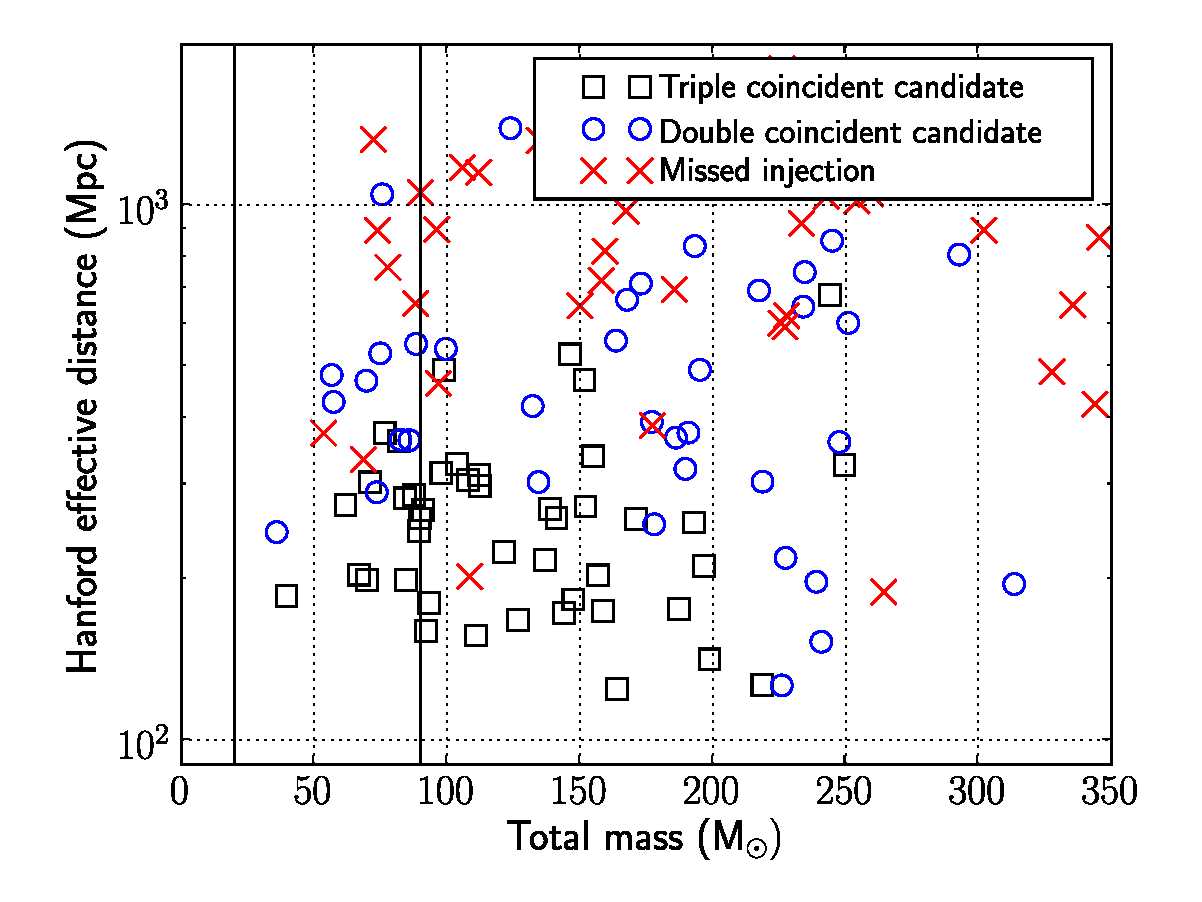
\includegraphics[width=0.49\textwidth]{figures/ninja1/spa_erd_3_5pn_found_missed_mchirp}
  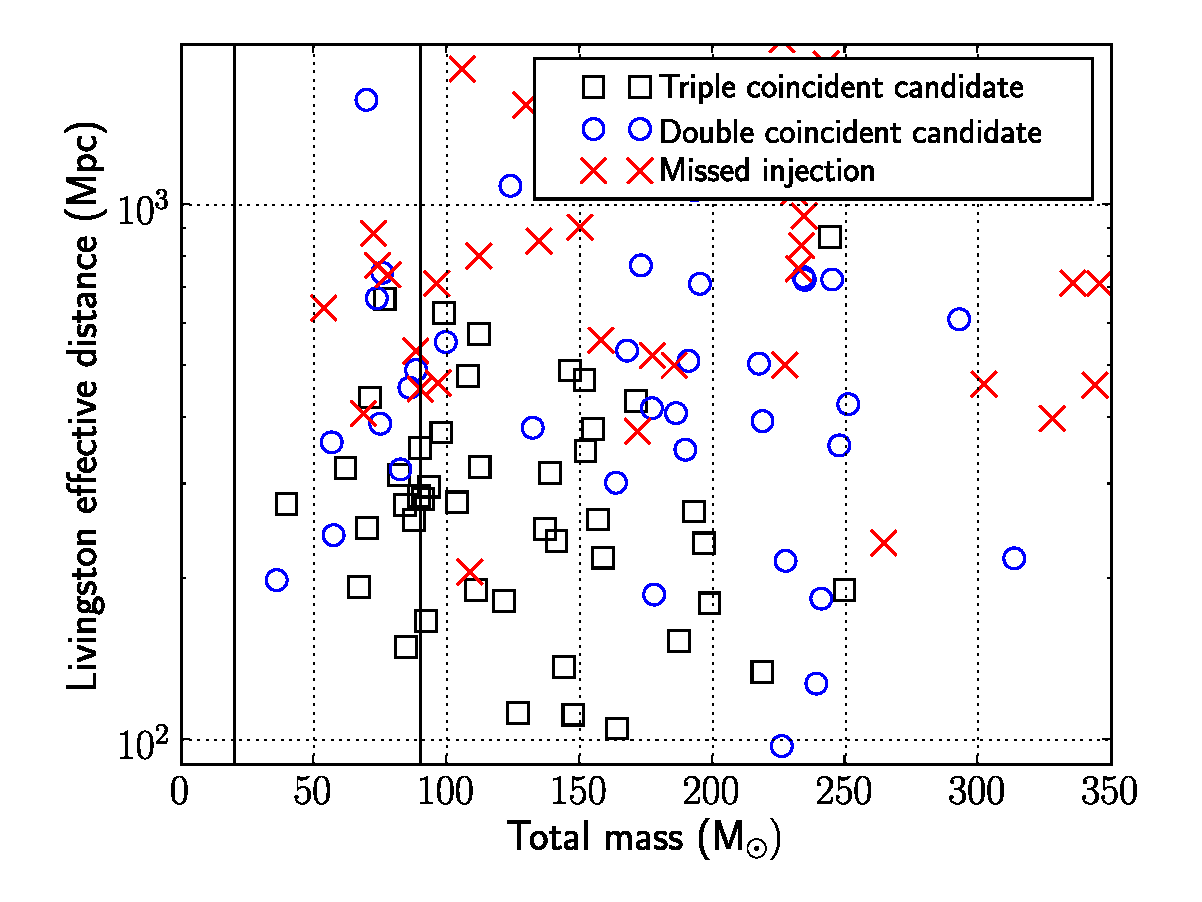
\includegraphics[width=0.49\textwidth]{figures/ninja1/spa_erd_3_5pn_found_missed_mchirp_l}
\end{center}
\caption{\textbf{Found and missed injections using TaylorF2 templates terminated at ERD}, plotted as a function
of the injected effective distance in Hanford (left) and Livingston (right) and the total mass of the injection. Since the LIGO Observatories are not exactly aligned, the effective distance of a signal can differ, depending on the sky location of the signal.
The vertical bars mark the limits of the template bank used in the search.  For
the lower masses, we see that the majority of the closer injections 
are found in coincidence in all three of
the detectors.  There is then a band of injections which are found only
in two detectors -- H1 and L1 and not the less sensitive H2 detector.
For higher masses, the results are less meaningful as the template bank
was only taken to a total mass of $90 M_{\odot}$.}
\label{fig:3_5pn_found_missed}
\end{figure}

Figure~\ref{fig:3_5pn_params} shows the accuracy with which the total mass and
coalescence time of the binary are recovered when using the 3.5 post-Newtonian
order Taylor F2 templates. The total mass fraction difference is computed as
$(M_\mathrm{injected} - M_\mathrm{detected})/ M_\mathrm{injected}$. For lower
mass signals, the end time is recovered reasonably accurately, with accuracy
decreasing for the high mass systems. The total mass recovery is poor for the
majority of signals, with good parameter estimation for only a few of the
lowest mass simulations.

\begin{figure}
    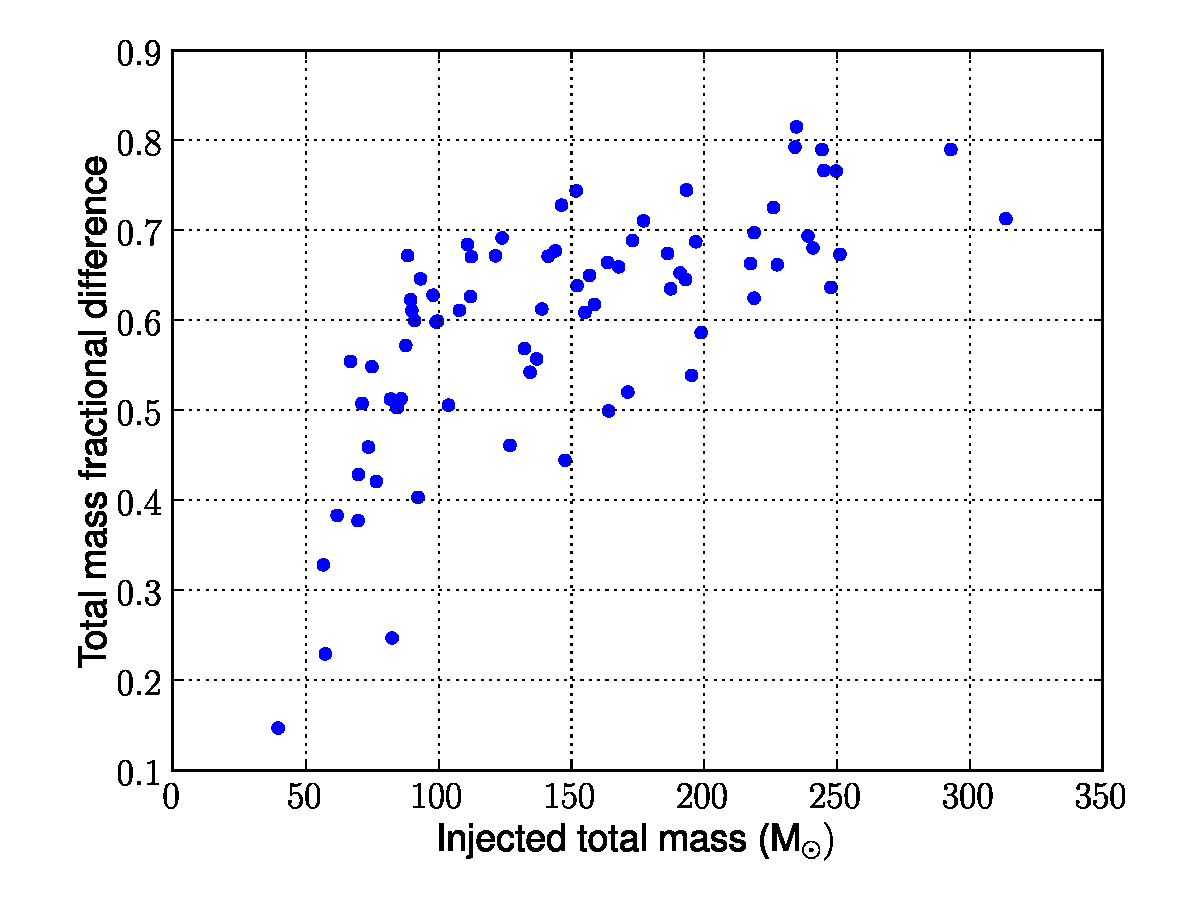
\includegraphics[width=0.50\textwidth]{figures/ninja1/spa_erd_3_5pn_mass_estimate}
    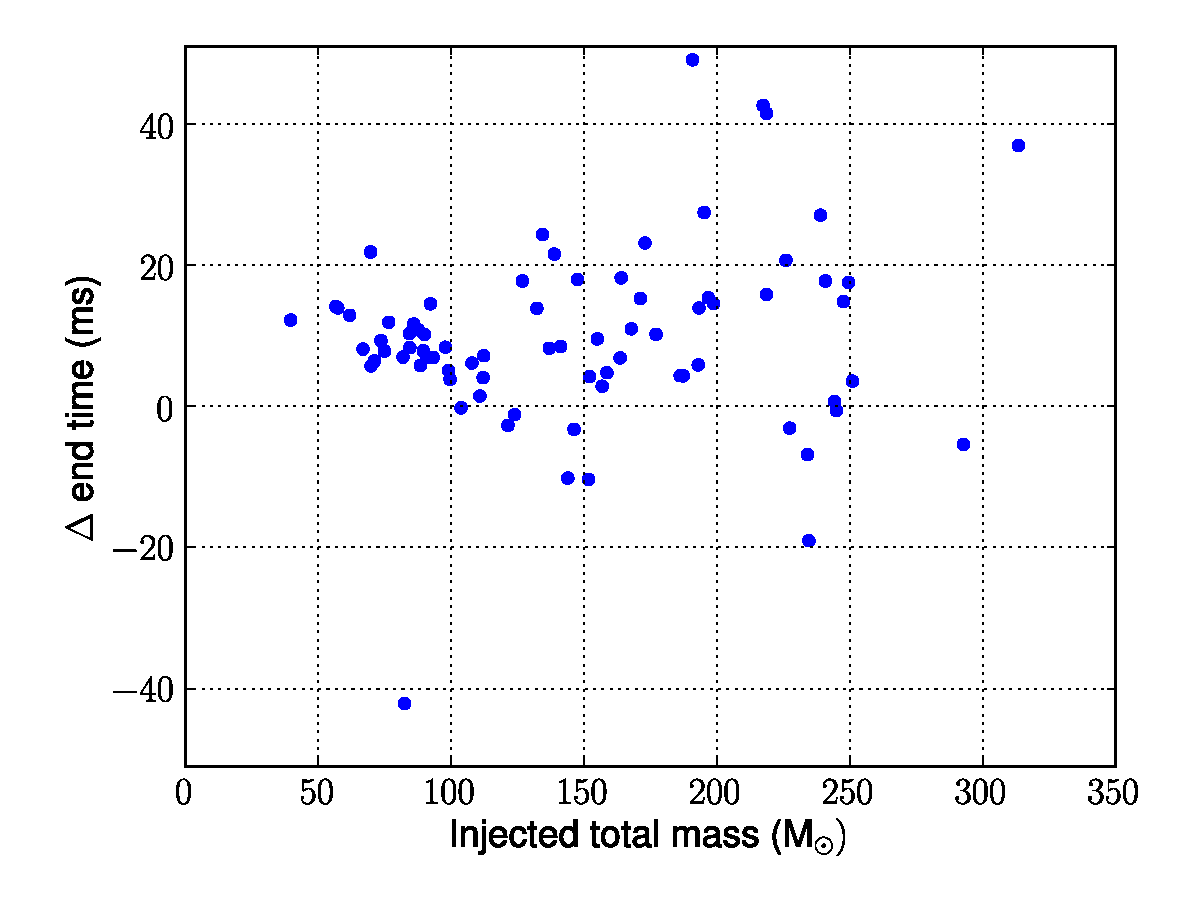
\includegraphics[width=0.50\textwidth]{figures/ninja1/spa_erd_3_5pn_time_estimate_vs_mt}
\caption{\textbf{Parameter accuracy using TaylorF2 templates terminated at
ERD}.\textbf{Left:} Accuracy with which the total mass is recovered. The
template bank covers the region $20 M_\odot \le M \le 90 M_\odot$, hence
the mass of injections with $M > 90 M_\odot$ are always underestimated.
Even within the region covered by the bank, the TaylorF2 templates
systematically underestimate the mass of the injected signals and the total
mass is recovered accurately only for a few injections.  The vast majority of
recoverd signals have an error of $40\%$ or greater. \textbf{Right:} Accuracy
of determining the coalescence time of the injections.  The end time is not
recovered accurately, the timing error can become as large as $50
\mathrm{ms}$, the limits of the injection window.  }
\label{fig:3_5pn_params}
\end{figure}






